%% Generated by Sphinx.
\def\sphinxdocclass{report}
\documentclass[a4paper,11pt,oneside,english,openany]{sphinxmanual}
\ifdefined\pdfpxdimen
   \let\sphinxpxdimen\pdfpxdimen\else\newdimen\sphinxpxdimen
\fi \sphinxpxdimen=.75bp\relax
\ifdefined\pdfimageresolution
    \pdfimageresolution= \numexpr \dimexpr1in\relax/\sphinxpxdimen\relax
\fi
%% let collapsible pdf bookmarks panel have high depth per default
\PassOptionsToPackage{bookmarksdepth=5}{hyperref}

\PassOptionsToPackage{booktabs}{sphinx}
\PassOptionsToPackage{colorrows}{sphinx}

\PassOptionsToPackage{warn}{textcomp}
\usepackage[utf8]{inputenc}
\ifdefined\DeclareUnicodeCharacter
% support both utf8 and utf8x syntaxes
  \ifdefined\DeclareUnicodeCharacterAsOptional
    \def\sphinxDUC#1{\DeclareUnicodeCharacter{"#1}}
  \else
    \let\sphinxDUC\DeclareUnicodeCharacter
  \fi
  \sphinxDUC{00A0}{\nobreakspace}
  \sphinxDUC{2500}{\sphinxunichar{2500}}
  \sphinxDUC{2502}{\sphinxunichar{2502}}
  \sphinxDUC{2514}{\sphinxunichar{2514}}
  \sphinxDUC{251C}{\sphinxunichar{251C}}
  \sphinxDUC{2572}{\textbackslash}
\fi
\usepackage{cmap}
\usepackage[T1]{fontenc}
\usepackage{amsmath,amssymb,amstext}
\usepackage{babel}





\usepackage[Bjarne]{fncychap}
\usepackage{sphinx}

\fvset{fontsize=auto}
\usepackage{geometry}


% Include hyperref last.
\usepackage{hyperref}
% Fix anchor placement for figures with captions.
\usepackage{hypcap}% it must be loaded after hyperref.
% Set up styles of URL: it should be placed after hyperref.
\urlstyle{same}

\addto\captionsenglish{\renewcommand{\contentsname}{Contents:}}

\usepackage{sphinxmessages}
\setcounter{tocdepth}{1}


		\renewcommand{\familydefault}{\rmdefault}
        \usepackage{setspace} % Required for more spacing options
		\parindent 0px
		\setstretch{1.3}
        \usepackage[T1]{fontenc}
        \usepackage{charter}
        \usepackage{amsmath}
        \usepackage{amsfonts}
        \usepackage{amssymb}
        \usepackage{fancyhdr}
        \usepackage{arydshln}
        \usepackage{xcolor}
        \usepackage{makeidx}  % To create an index
        \usepackage{tocloft}  % To customize Table of Contents

        % Fancy header and footer
        \pagestyle{fancy}
        \fancyhead[L]{\leftmark}
        \fancyhead[R]{\thepage}
        \fancyfoot[C]{}

        % Table of Contents: Formatting (removing subsections)
        \setcounter{tocdepth}{1}  % Limit ToC to sections only (remove subsections)
        \renewcommand{\cftsecfont}{\normalfont\bfseries}  % Bold section titles
        \renewcommand{\cftsecindent}{0em}                 % No indentation for sections
        \setlength{\cftbeforesecskip}{0.5ex}              % Space before section titles

        % Index Configuration (simplified to sections only)
        \makeindex  % Generate index

        % Page layout adjustments
		\usepackage{geometry}
        \geometry{top=1.5cm, bottom=1.5cm, left=1.3cm, right=1.3cm}
        \usepackage{hyperref}
        \hypersetup{colorlinks=true,linkcolor=violet,filecolor=magenta,urlcolor=blue}

        % Better verbatim environment for code blocks
        %\usepackage{fvextra}
        \usepackage{tcolorbox}
        
        \newtcbox{\tbox}{colframe=black,colback=gray!5,boxrule=0.7pt,arc=4pt,boxsep=5pt}
    

\title{Power Spectrum Estimation}
\date{Jun 01, 2026}
\release{1.0.0}
\author{AE,SB,BB}
\newcommand{\sphinxlogo}{\vbox{}}
\renewcommand{\releasename}{Release}
\makeindex
\begin{document}

\ifdefined\shorthandoff
  \ifnum\catcode`\=\string=\active\shorthandoff{=}\fi
  \ifnum\catcode`\"=\active\shorthandoff{"}\fi
\fi

\pagestyle{empty}
\sphinxmaketitle
\pagestyle{plain}
\sphinxtableofcontents
\pagestyle{normal}
\phantomsection\label{\detokenize{index::doc}}
\sphinxstepscope



\sphinxstepscope


\chapter{psestimation module}
\label{\detokenize{psestimation:module-psestimation}}\label{\detokenize{psestimation:psestimation-module}}\label{\detokenize{psestimation::doc}}\index{module@\spxentry{module}!psestimation@\spxentry{psestimation}}\index{psestimation@\spxentry{psestimation}!module@\spxentry{module}}
\begin{table}[htbp]
  \centering
  \footnotesize
  \setlength{\tabcolsep}{20pt}
  \setlength{\arrayrulewidth}{0.5pt}

  \renewcommand{\arraystretch}{1.9}
  \setlength{\doublerulesep}{1.3pt}  % <-- reduce space between double lines
  \scalebox{1}{
    \begin{tabular}{||p{7.cm}|l|l||}
      \hline\hline
      Quantity & Mathematical symbol & Codespace name \\
      \hline\hline
      Centered frequency & $\nu_c$ & \texttt{nuc}\\ \hline
      Separation between two frequency channels & $\Delta\nu_c$ & \texttt{dnuc}\\ \hline
      Number of frequency separations used to estimate cylindrical power spectrum & $N_E$ & \texttt{NE}\\\hline
      Comoving distance at $\nu_c$   & $r$ & \texttt{r}\\ \hline
      Derivative of comoving distance w.r.t. frequency $\nu$, evaluated at $\nu_c$ & $r^{\prime} = \left.\frac{dr}{d\nu}\right|_{\nu_c}$ & \texttt{rp}\\ \hline
      Slope of Wedge boundary line & $\frac{[k_{\parallel}]_H}{k_{\perp}} = \frac{r}{r^{\prime}\nu_c}$ & \texttt{fac}\\ \hline
      Prefactor in Fourier Transform (\textit{volume factor}) & $r^2r'\Delta\nu_c(N_E-1)$ & \texttt{vfac}\\ \hline
      Component of $\vec{\bf k}$ perpendicular to line of sight & $k_{\perp}$ & \texttt{kper}\\ \hline
      Component of $\vec{\bf k}$ parallel to line of sight & $k_{\parallel}$ & \texttt{kpara}\\ \hline
      Multi-angular power spectrum (MAPS )& $C_{\ell}(\Delta\nu)$ & \texttt{cl}\\ \hline
      Cylindrical power spectrum & $P(k_{\perp},k_{\parallel})$ & \texttt{pk}\\ \hline
      Standard deviation of $P_{N}(k_{\perp},k_{\parallel})$ & $\delta P_{N}(k_{\perp},k_{\parallel})$ & \texttt{dpkn}\\ \hline
      Mean of variable $X$ & $\mu_{\rm Est}$ & \texttt{mu\_est} \\ \hline
      Standard deviation of variable $X$ & $\sigma_{\rm Est}$ & \texttt{sigma\_est} \\ \hline
      Scaled std of $P_{N}(k_{\perp},k_{\parallel})$ & $\delta P_{N}^{True}(k_{\perp},k_{\parallel}) = \sigma_{\rm Est}\,\delta P_{N}(k_{\perp},k_{\parallel})$ & \texttt{dpk}\\ \hline
      Number of logarithmic bins & $N_{\rm Bin}$         & \texttt{NBin}\\ \hline
      Binned $k$ values      & $k$                       & \texttt{kk/keff}\\ \hline
      Binned power spectrum  & $P(k)$                    & \texttt{ppk}\\ \hline
      Error in estimating binned power spectrum          & $\delta P(k)$                       & \texttt{dppk}\\ \hline
      Dimensionless power spectrum & $\Delta^2(k)$ & \texttt{dk2}\\ \hline
      $2\sigma$ uncertainty of $\Delta^2(k)$ & $2\sigma(k)$ & \texttt{dpk2}\\ \hline
      Signal to noise ratio & $\textsc{SNR} = \Delta^2(k)/\sigma(k)$ & \texttt{snr} \\ \hline
      Upper limits of power spectrum & $\Delta^2_{\text{UL}}(k)$ & \texttt{ul}\\
      \hline\hline
    \end{tabular}
  }
  \caption{Namespace convensions}
  \label{tab:f_outputs}
\end{table}
\clearpage
\index{build\_essential() (in module psestimation)@\spxentry{build\_essential()}\spxextra{in module psestimation}}

\begin{fulllineitems}
\phantomsection\label{\detokenize{psestimation:psestimation.build_essential}}
\pysigstartsignatures
\pysiglinewithargsret{\sphinxcode{\sphinxupquote{psestimation.}}\sphinxbfcode{\sphinxupquote{build\_essential}}}{\sphinxparam{\DUrole{n}{nuc}}\sphinxparamcomma \sphinxparam{\DUrole{n}{dnuc}}\sphinxparamcomma \sphinxparam{\DUrole{n}{NE}}\sphinxparamcomma \sphinxparam{\DUrole{n}{lval}}\sphinxparamcomma \sphinxparam{\DUrole{n}{model}\DUrole{o}{=}\DUrole{default_value}{\textquotesingle{}Planck18\textquotesingle{}}}}{}
\pysigstopsignatures
\sphinxAtStartPar
For a given set of values \(\nu_c,\Delta\nu_c,N_E,\ell\) and appropriate cosmological model either \sphinxstylestrong{Planck18} or \sphinxstylestrong{FlatLambdaCDM}, it calculates  comoving distance \(r\) at \(\nu_c\) and it’s frequency derivative \(r^\prime\). It also calculates the slope of wedge boundary line, corresponding volume factor, and components of \(\vec{\mathbf{k}}\): \(k_{\perp}\,\text{and}\,k_{\parallel}\) respectively.
\begin{quote}\begin{description}
\sphinxlineitem{Parameters}\begin{itemize}
\item {} 
\sphinxAtStartPar
\sphinxstyleliteralstrong{\sphinxupquote{nuc}} (\sphinxstyleliteralemphasis{\sphinxupquote{float}}) \textendash{} Central frequency \(\nu_c\) in units of \(\rm MHz\).

\item {} 
\sphinxAtStartPar
\sphinxstyleliteralstrong{\sphinxupquote{dnuc}} (\sphinxstyleliteralemphasis{\sphinxupquote{float}}) \textendash{} Separation between two frequency channels \(\Delta\nu_c\) in units of \(\rm MHz\).

\item {} 
\sphinxAtStartPar
\sphinxstyleliteralstrong{\sphinxupquote{NE}} (\sphinxstyleliteralemphasis{\sphinxupquote{int}}) \textendash{} Number of frequency separations used in the analysis \(N_E\).

\item {} 
\sphinxAtStartPar
\sphinxstyleliteralstrong{\sphinxupquote{lval}} (\sphinxstyleliteralemphasis{\sphinxupquote{np.ndarray}}) \textendash{} Angular multipole \(\ell\) values.

\item {} 
\sphinxAtStartPar
\sphinxstyleliteralstrong{\sphinxupquote{model}} (\sphinxstyleliteralemphasis{\sphinxupquote{str \{\textquotesingle{}Planck18\textquotesingle{}}}\sphinxstyleliteralemphasis{\sphinxupquote{,}}\sphinxstyleliteralemphasis{\sphinxupquote{\textquotesingle{}FlatLambdaCDM\textquotesingle{}\}}}\sphinxstyleliteralemphasis{\sphinxupquote{, }}\sphinxstyleliteralemphasis{\sphinxupquote{optional}}) \textendash{} The name of cosmological model used to calculate \sphinxstylestrong{comoving distance} \(r\). By default \sphinxstylestrong{Planck18} is used.

\end{itemize}

\sphinxlineitem{Returns}
\sphinxAtStartPar
\begin{itemize}
\item {} 
\sphinxAtStartPar
\sphinxstylestrong{r} (\sphinxstyleemphasis{float}) \textendash{} Comoving distance \(r\) at \(\nu_c\) in units of \(\rm Mpc\).

\item {} 
\sphinxAtStartPar
\sphinxstylestrong{rp} (\sphinxstyleemphasis{float}) \textendash{} Derivative of comoving distance \(r\) w.r.t. frequency \(\nu\), evaluated at \(\nu_c\), \(r^{\prime} = \left.\frac{dr}{d\nu}\right|_{\nu_c}\approx \tfrac{c}{H(z)}\times\tfrac{(1+z)^2}{\nu_e = \mathbf{1420\,\rm MHz}}\) in units of \(\rm Mpc/MHz\).

\item {} 
\sphinxAtStartPar
\sphinxstylestrong{fac} (\sphinxstyleemphasis{float}) \textendash{} Slope of Wedge boundary line  \([k_{\parallel}]_H = [r/{r^{\prime}\nu_c}]\, k_{\perp}\).

\item {} 
\sphinxAtStartPar
\sphinxstylestrong{vfac} (\sphinxstyleemphasis{float}) \textendash{} Factor (\sphinxstylestrong{volume factor}) in Fourier Transform, \(r^2r^{\prime}\Delta\nu_c(N_E-1)\).

\item {} 
\sphinxAtStartPar
\sphinxstylestrong{kper} (\sphinxstyleemphasis{np.ndarray}) \textendash{} Component of \(\vec{\bf k}\), perpendicular to line of sight, \(k_{\perp} = \ell/r\).

\item {} 
\sphinxAtStartPar
\sphinxstylestrong{kpara} (\sphinxstyleemphasis{np.ndarray}) \textendash{} Component of \(\vec{\bf k}\), parallel to line of sight, with :

\begin{center}
    \tbox{$k_{\parallel m} = \dfrac{\pi m}{r^{\prime}\Delta\nu_c(N_E-1)},\quad m = 0,1,\dots,N_E-1.$}
\end{center}

\clearpage

\end{itemize}


\end{description}\end{quote}
\subsubsection*{Examples}

\begin{sphinxVerbatim}[commandchars=\\\{\}]
\PYG{g+gp}{\PYGZgt{}\PYGZgt{}\PYGZgt{} }\PYG{k+kn}{import} \PYG{n+nn}{numpy} \PYG{k}{as} \PYG{n+nn}{np}
\PYG{g+gp}{\PYGZgt{}\PYGZgt{}\PYGZgt{} }\PYG{k+kn}{import} \PYG{n+nn}{myutils}\PYG{n+nn}{.}\PYG{n+nn}{psfuncs}\PYG{n+nn}{.}\PYG{n+nn}{psestimation} \PYG{k}{as} \PYG{n+nn}{pe}
\PYG{g+go}{Imported myutils}
\PYG{g+go}{Imported psfuncs,   Import Time : 01/06/26 | 04:05:54 PM}
\PYG{g+gp}{\PYGZgt{}\PYGZgt{}\PYGZgt{} }\PYG{n}{nuc}  \PYG{o}{=} \PYG{l+m+mf}{154.255} \PYG{c+c1}{\PYGZsh{} observing frequency in MHz}
\PYG{g+gp}{\PYGZgt{}\PYGZgt{}\PYGZgt{} }\PYG{n}{dnuc} \PYG{o}{=} \PYG{l+m+mf}{0.04}    \PYG{c+c1}{\PYGZsh{} freq separation in MHz}
\PYG{g+gp}{\PYGZgt{}\PYGZgt{}\PYGZgt{} }\PYG{n}{NE}   \PYG{o}{=} \PYG{l+m+mi}{668}     \PYG{c+c1}{\PYGZsh{} no of channels used to estimate PS}
\PYG{g+gp}{\PYGZgt{}\PYGZgt{}\PYGZgt{} }\PYG{c+c1}{\PYGZsh{} ell values array}
\PYG{g+gp}{\PYGZgt{}\PYGZgt{}\PYGZgt{} }\PYG{n}{fname} \PYG{o}{=} \PYG{l+s+s1}{\PYGZsq{}}\PYG{l+s+s1}{/home/cts23ph/git\PYGZus{}package\PYGZus{}myutils/tge/bin\PYGZus{}info\PYGZus{}1000007200.npz}\PYG{l+s+s1}{\PYGZsq{}}
\PYG{g+gp}{\PYGZgt{}\PYGZgt{}\PYGZgt{} }\PYG{n}{lval}  \PYG{o}{=} \PYG{p}{(}\PYG{n}{np}\PYG{o}{.}\PYG{n}{load}\PYG{p}{(}\PYG{n}{fname}\PYG{p}{)}\PYG{p}{[}\PYG{l+s+s1}{\PYGZsq{}}\PYG{l+s+s1}{lval}\PYG{l+s+s1}{\PYGZsq{}}\PYG{p}{]}\PYG{p}{)}\PYG{o}{.}\PYG{n}{astype}\PYG{p}{(}\PYG{l+s+s1}{\PYGZsq{}}\PYG{l+s+s1}{int}\PYG{l+s+s1}{\PYGZsq{}}\PYG{p}{)}
\PYG{g+gp}{\PYGZgt{}\PYGZgt{}\PYGZgt{} }\PYG{n}{r}\PYG{p}{,} \PYG{n}{rp}\PYG{p}{,} \PYG{n}{fac}\PYG{p}{,} \PYG{n}{vfac}\PYG{p}{,} \PYG{n}{kper}\PYG{p}{,} \PYG{n}{kpara} \PYG{o}{=} \PYG{n}{pe}\PYG{o}{.}\PYG{n}{build\PYGZus{}essential}\PYG{p}{(}\PYG{n}{nuc}\PYG{p}{,} \PYG{n}{dnuc}\PYG{p}{,} \PYG{n}{NE}\PYG{p}{,} \PYG{n}{lval}\PYG{p}{)}
\PYG{g+go}{\PYGZhy{}\PYGZhy{}\PYGZhy{}\PYGZhy{}\PYGZhy{}\PYGZhy{}\PYGZhy{}\PYGZhy{}\PYGZhy{}\PYGZhy{}\PYGZhy{}\PYGZhy{}\PYGZhy{}\PYGZhy{}\PYGZhy{}\PYGZhy{}\PYGZhy{}\PYGZhy{}\PYGZhy{}\PYGZhy{}\PYGZhy{}\PYGZhy{}\PYGZhy{}\PYGZhy{}\PYGZhy{}\PYGZhy{}\PYGZhy{}\PYGZhy{}\PYGZhy{}\PYGZhy{}\PYGZhy{}\PYGZhy{}\PYGZhy{}\PYGZhy{}\PYGZhy{}\PYGZhy{}\PYGZhy{}\PYGZhy{}}
\PYG{g+go}{Cosmological Model: Planck18}
\PYG{g+go}{Redshift          : z  = 8.21}
\PYG{g+go}{Comoving distance : r  = 9191.20 Mpc}
\PYG{g+go}{rprime            : rp = 16.93 Mpc/MHz}
\PYG{g+go}{Sep used          : NE = 668}
\PYG{g+go}{\PYGZhy{}\PYGZhy{}\PYGZhy{}\PYGZhy{}\PYGZhy{}\PYGZhy{}\PYGZhy{}\PYGZhy{}\PYGZhy{}\PYGZhy{}\PYGZhy{}\PYGZhy{}\PYGZhy{}\PYGZhy{}\PYGZhy{}\PYGZhy{}\PYGZhy{}\PYGZhy{}\PYGZhy{}\PYGZhy{}\PYGZhy{}\PYGZhy{}\PYGZhy{}\PYGZhy{}\PYGZhy{}\PYGZhy{}\PYGZhy{}\PYGZhy{}\PYGZhy{}\PYGZhy{}\PYGZhy{}\PYGZhy{}\PYGZhy{}\PYGZhy{}\PYGZhy{}\PYGZhy{}\PYGZhy{}\PYGZhy{}}
\PYG{g+go}{Wedge boundary slope (fac) : 3.519}
\PYG{g+go}{DCT factor (vfac)          : 3.816e+10}
\PYG{g+go}{kper.shape                 : (20,)}
\PYG{g+go}{kpara.shape                : (668,)}
\PYG{g+go}{\PYGZhy{}\PYGZhy{}\PYGZhy{}\PYGZhy{}\PYGZhy{}\PYGZhy{}\PYGZhy{}\PYGZhy{}\PYGZhy{}\PYGZhy{}\PYGZhy{}\PYGZhy{}\PYGZhy{}\PYGZhy{}\PYGZhy{}\PYGZhy{}\PYGZhy{}\PYGZhy{}\PYGZhy{}\PYGZhy{}\PYGZhy{}\PYGZhy{}\PYGZhy{}\PYGZhy{}\PYGZhy{}\PYGZhy{}\PYGZhy{}\PYGZhy{}\PYGZhy{}\PYGZhy{}\PYGZhy{}\PYGZhy{}\PYGZhy{}\PYGZhy{}\PYGZhy{}\PYGZhy{}\PYGZhy{}\PYGZhy{}}
\end{sphinxVerbatim}

\begin{sphinxVerbatim}[commandchars=\\\{\}]
\PYG{g+gp}{\PYGZgt{}\PYGZgt{}\PYGZgt{} }\PYG{n}{r}\PYG{p}{,} \PYG{n}{rp}\PYG{p}{,} \PYG{n}{fac}\PYG{p}{,} \PYG{n}{vfac}\PYG{p}{,} \PYG{n}{kper}\PYG{p}{,} \PYG{n}{kpara} \PYG{o}{=} \PYG{n}{pe}\PYG{o}{.}\PYG{n}{build\PYGZus{}essential}\PYG{p}{(}\PYG{n}{nuc}\PYG{p}{,} \PYG{n}{dnuc}\PYG{p}{,} \PYG{n}{NE}\PYG{p}{,} \PYG{n}{lval}\PYG{p}{,}
\PYG{g+gp}{... }                                                     \PYG{n}{model} \PYG{o}{=} \PYG{l+s+s1}{\PYGZsq{}}\PYG{l+s+s1}{FlatLambdaCDM}\PYG{l+s+s1}{\PYGZsq{}}\PYG{p}{)}
\PYG{g+go}{\PYGZhy{}\PYGZhy{}\PYGZhy{}\PYGZhy{}\PYGZhy{}\PYGZhy{}\PYGZhy{}\PYGZhy{}\PYGZhy{}\PYGZhy{}\PYGZhy{}\PYGZhy{}\PYGZhy{}\PYGZhy{}\PYGZhy{}\PYGZhy{}\PYGZhy{}\PYGZhy{}\PYGZhy{}\PYGZhy{}\PYGZhy{}\PYGZhy{}\PYGZhy{}\PYGZhy{}\PYGZhy{}\PYGZhy{}\PYGZhy{}\PYGZhy{}\PYGZhy{}\PYGZhy{}\PYGZhy{}\PYGZhy{}\PYGZhy{}\PYGZhy{}\PYGZhy{}\PYGZhy{}\PYGZhy{}\PYGZhy{}}
\PYG{g+go}{Cosmological Model: FlatLambdaCDM}
\PYG{g+go}{Redshift          : z  = 8.21}
\PYG{g+go}{Comoving distance : r  = 9209.37 Mpc}
\PYG{g+go}{rprime            : rp = 16.99 Mpc/MHz}
\PYG{g+go}{Sep used          : NE = 668}
\PYG{g+go}{\PYGZhy{}\PYGZhy{}\PYGZhy{}\PYGZhy{}\PYGZhy{}\PYGZhy{}\PYGZhy{}\PYGZhy{}\PYGZhy{}\PYGZhy{}\PYGZhy{}\PYGZhy{}\PYGZhy{}\PYGZhy{}\PYGZhy{}\PYGZhy{}\PYGZhy{}\PYGZhy{}\PYGZhy{}\PYGZhy{}\PYGZhy{}\PYGZhy{}\PYGZhy{}\PYGZhy{}\PYGZhy{}\PYGZhy{}\PYGZhy{}\PYGZhy{}\PYGZhy{}\PYGZhy{}\PYGZhy{}\PYGZhy{}\PYGZhy{}\PYGZhy{}\PYGZhy{}\PYGZhy{}\PYGZhy{}\PYGZhy{}}
\PYG{g+go}{Wedge boundary slope (fac) : 3.514}
\PYG{g+go}{DCT factor (vfac)          : 3.844e+10}
\PYG{g+go}{kper.shape                 : (20,)}
\PYG{g+go}{kpara.shape                : (668,)}
\PYG{g+go}{\PYGZhy{}\PYGZhy{}\PYGZhy{}\PYGZhy{}\PYGZhy{}\PYGZhy{}\PYGZhy{}\PYGZhy{}\PYGZhy{}\PYGZhy{}\PYGZhy{}\PYGZhy{}\PYGZhy{}\PYGZhy{}\PYGZhy{}\PYGZhy{}\PYGZhy{}\PYGZhy{}\PYGZhy{}\PYGZhy{}\PYGZhy{}\PYGZhy{}\PYGZhy{}\PYGZhy{}\PYGZhy{}\PYGZhy{}\PYGZhy{}\PYGZhy{}\PYGZhy{}\PYGZhy{}\PYGZhy{}\PYGZhy{}\PYGZhy{}\PYGZhy{}\PYGZhy{}\PYGZhy{}\PYGZhy{}\PYGZhy{}}
\PYG{g+gp}{\PYGZgt{}\PYGZgt{}\PYGZgt{} }\PYG{c+c1}{\PYGZsh{} kper  shape (len(lval),)}
\PYG{g+gp}{\PYGZgt{}\PYGZgt{}\PYGZgt{} }\PYG{c+c1}{\PYGZsh{} kpara shape (NE,)}
\end{sphinxVerbatim}

\clearpage
\subsubsection*{Notes}

\sphinxAtStartPar
For calculating comoving distance \(r\), we use \sphinxstylestrong{Flat} \(\Lambda\rm CDM\) cosmological model. The cosmological parameters are from either from \sphinxhref{https://arxiv.org/abs/1807.06209}{Planck 2018 results. VI. Cosmological parameters}  or \sphinxstylestrong{FlatLambdaCDM}. The \sphinxhref{https://docs.astropy.org/en/latest/api/astropy.cosmology.realizations.Planck18.html}{Planck 18 Astropy} , \sphinxhref{https://docs.astropy.org/en/latest/api/astropy.cosmology.FlatLambdaCDM.html}{FlatLambdaCDM} and module have been used here.
\begin{enumerate}
\sphinxsetlistlabels{\arabic}{enumi}{enumii}{}{.}%
\item {} 
\sphinxAtStartPar
For \sphinxstylestrong{Planck18} we have :
\begin{quote}

\begin{table}[h]
  \centering
  \footnotesize
  \setlength{\tabcolsep}{15pt}
  \setlength{\arrayrulewidth}{0.1pt}

  \renewcommand{\arraystretch}{1.7}
  \setlength{\doublerulesep}{1pt}  % <-- reduce space between double lines
  \scalebox{1}{
    \begin{tabular}{||l||c||c||}
      \hline\hline
      \multicolumn{1}{||c||}{Quantity} & \multicolumn{1}{|c||}{Mathematical symbol} & \multicolumn{1}{|c||}{Value} \\
      \hline\hline
      Hubble Constant at present & $H_{0}$ & $67.66\,\rm km/s/Mpc$ \\ \hline
      Density parameter of matter & $\Omega_{m\displaystyle 0}$ & $0.30966$ \\ \hline
      Density parameter of baryonic matter & $\Omega_{b\displaystyle 0}$ & $0.04897$ \\ \hline
      CMB temperature at present & $T_{{\scriptscriptstyle \mathrm{CMB}}\displaystyle 0}$ & $2.7255 K$ \\ \hline
      Effective number of neutino species & $N_{\rm eff}$ & $3.046$\\ \hline
      Mass of neutrinos & $m_{\nu}$ & $[0, 0, 0.06]\, \rm eV$ \\
      \hline\hline
      \end{tabular}
  }
  \caption{Cosmological parameters taken from {\href{https://arxiv.org/abs/1807.06209}{\bf Planck 18}} used by {\href{https://docs.astropy.org/en/latest/api/astropy.cosmology.realizations.Planck18.html}{\bf Astropy module}}.}
  \label{tab:cosmo}
\end{table}
\vspace{-1cm}
\end{quote}

\item {} 
\sphinxAtStartPar
For \sphinxstylestrong{FlatLambdaCDM} model we have considered that there is no curvature, \(\Omega_{k0} = 0\). In this, we have assumed that \sphinxstylestrong{matter and dark energy} are the only constituents of the Universe. Here we have taken the corresponding desity parameters \(\Omega_{m\displaystyle 0} = 0.30966, \Omega_{\Lambda\displaystyle 0} = 0.69034, \Omega_{\rm total\displaystyle 0} = \Omega_{m\displaystyle 0} + \Omega_{\Lambda\displaystyle 0} = 1\). And the present value of \sphinxstylestrong{Hubble constant} is \(H_{0} = 67.66\,\rm km/s/Mpc\).

\end{enumerate}

\clearpage

\end{fulllineitems}

\index{calc\_A() (in module psestimation)@\spxentry{calc\_A()}\spxextra{in module psestimation}}

\begin{fulllineitems}
\phantomsection\label{\detokenize{psestimation:psestimation.calc_A}}
\pysigstartsignatures
\pysiglinewithargsret{\sphinxcode{\sphinxupquote{psestimation.}}\sphinxbfcode{\sphinxupquote{calc\_A}}}{\sphinxparam{\DUrole{n}{na}}\sphinxparamcomma \sphinxparam{\DUrole{n}{nb}}}{}
\pysigstopsignatures\begin{quote}\begin{description}
\sphinxlineitem{Parameters}\begin{itemize}
\item {} 
\sphinxAtStartPar
\sphinxstyleliteralstrong{\sphinxupquote{na}} (\sphinxstyleliteralemphasis{\sphinxupquote{int}}) \textendash{} Non negative integer greater than 2.

\item {} 
\sphinxAtStartPar
\sphinxstyleliteralstrong{\sphinxupquote{nb}} (\sphinxstyleliteralemphasis{\sphinxupquote{int}}) \textendash{} Non negative integer greater than 2.

\end{itemize}

\sphinxlineitem{Returns}
\sphinxAtStartPar

\sphinxAtStartPar
\sphinxstylestrong{A} \textendash{} A 2D matrix of shape \((na\times nb)\), with
\begin{center}
\tbox{$A_{\rho\lambda} = B_{\rho\lambda}\,\cos\left(\dfrac{\pi\rho\lambda}{nb-1}\right)$}
\end{center}
\sphinxAtStartPar
Where \(\rho = 0,1,\dots,(na-1)\), \(\lambda = 0,1,\dots,(nb-1)\)
\begin{center}
        \tbox{$
B_{\rho\lambda} =
\begin{cases}
        0.5 & \text{if } \lambda = 0 \text{ or } (nb-1) \\
    1.0 & \text{otherwise}
\end{cases}$}
\end{center}

\sphinxlineitem{Return type}
\sphinxAtStartPar
np.ndarray

\end{description}\end{quote}
\subsubsection*{Examples}

\begin{sphinxVerbatim}[commandchars=\\\{\}]
\PYG{g+gp}{\PYGZgt{}\PYGZgt{}\PYGZgt{} }\PYG{n+nb}{print}\PYG{p}{(}\PYG{n}{pe}\PYG{o}{.}\PYG{n}{calc\PYGZus{}A}\PYG{p}{(}\PYG{l+m+mi}{2}\PYG{p}{,}\PYG{l+m+mi}{2}\PYG{p}{)}\PYG{p}{)}
\PYG{g+go}{[[ 0.5  0.5]}
\PYG{g+go}{ [ 0.5 \PYGZhy{}0.5]]}
\PYG{g+gp}{\PYGZgt{}\PYGZgt{}\PYGZgt{} }\PYG{n+nb}{print}\PYG{p}{(}\PYG{n}{np}\PYG{o}{.}\PYG{n}{round}\PYG{p}{(}\PYG{n}{pe}\PYG{o}{.}\PYG{n}{calc\PYGZus{}A}\PYG{p}{(}\PYG{l+m+mi}{3}\PYG{p}{,}\PYG{l+m+mi}{3}\PYG{p}{)}\PYG{p}{,}\PYG{l+m+mi}{3}\PYG{p}{)}\PYG{p}{)}
\PYG{g+go}{[[ 0.5  1.   0.5]}
\PYG{g+go}{ [ 0.5  0.  \PYGZhy{}0.5]}
\PYG{g+go}{ [ 0.5 \PYGZhy{}1.   0.5]]}
\PYG{g+gp}{\PYGZgt{}\PYGZgt{}\PYGZgt{} }\PYG{n+nb}{print}\PYG{p}{(}\PYG{n}{np}\PYG{o}{.}\PYG{n}{round}\PYG{p}{(}\PYG{n}{pe}\PYG{o}{.}\PYG{n}{calc\PYGZus{}A}\PYG{p}{(}\PYG{l+m+mi}{4}\PYG{p}{,}\PYG{l+m+mi}{4}\PYG{p}{)}\PYG{p}{,}\PYG{l+m+mi}{3}\PYG{p}{)}\PYG{p}{)}
\PYG{g+go}{[[ 0.5  1.   1.   0.5]}
\PYG{g+go}{ [ 0.5  0.5 \PYGZhy{}0.5 \PYGZhy{}0.5]}
\PYG{g+go}{ [ 0.5 \PYGZhy{}0.5 \PYGZhy{}0.5  0.5]}
\PYG{g+go}{ [ 0.5 \PYGZhy{}1.   1.  \PYGZhy{}0.5]]}
\PYG{g+gp}{\PYGZgt{}\PYGZgt{}\PYGZgt{} }\PYG{n+nb}{print}\PYG{p}{(}\PYG{n}{np}\PYG{o}{.}\PYG{n}{round}\PYG{p}{(}\PYG{n}{pe}\PYG{o}{.}\PYG{n}{calc\PYGZus{}A}\PYG{p}{(}\PYG{l+m+mi}{2}\PYG{p}{,}\PYG{l+m+mi}{4}\PYG{p}{)}\PYG{p}{,}\PYG{l+m+mi}{3}\PYG{p}{)}\PYG{p}{)}
\PYG{g+go}{[[ 0.5  1.   1.   0.5]}
\PYG{g+go}{ [ 0.5  0.5 \PYGZhy{}0.5 \PYGZhy{}0.5]]}
\end{sphinxVerbatim}
\begin{quote}

\clearpage
\end{quote}

\end{fulllineitems}

\index{window() (in module psestimation)@\spxentry{window()}\spxextra{in module psestimation}}

\begin{fulllineitems}
\phantomsection\label{\detokenize{psestimation:psestimation.window}}
\pysigstartsignatures
\pysiglinewithargsret{\sphinxcode{\sphinxupquote{psestimation.}}\sphinxbfcode{\sphinxupquote{window}}}{\sphinxparam{\DUrole{n}{N}}}{}
\pysigstopsignatures
\sphinxAtStartPar
Returns a 4 term \sphinxstylestrong{Blackman\sphinxhyphen{}Nuttall} window function values.

\begin{center}
 \tbox{$F(a) = c_0 - c_1\,\cos\left(\dfrac{2\pi a}{2N-2}\right)+c_2\,\cos\left(\dfrac{4\pi a}{2N-2}\right)- c_3\,\cos\left(\dfrac{6\pi a}{2N-2}\right)\,\quad a = 0,1,\dots,2N-3$}
 \end{center}

\sphinxAtStartPar
Where
\begin{equation*}
\begin{split}c_0 = 0.3635819,c_1 = 0.4891775,c_2 = 0.1365995,c_3 = 0.0106411\end{split}
\end{equation*}
\sphinxAtStartPar
It has following properties :
\begin{equation*}
\begin{split}\boxed{F\Bigl[(N-1)+a\Bigr]=F\Bigl[(N-1)-a\Bigr]}\end{split}
\end{equation*}
\sphinxAtStartPar
and it’s also a periodic function with period \(2N-2\), i.e.
\begin{equation*}
\begin{split}\boxed{F\Bigl[a+\gamma(2N-2)\Bigr] = F(a),\quad \text{\rm with } \gamma = \pm1,\pm2,\dots}\end{split}
\end{equation*}
\sphinxAtStartPar
\(a = 0,1,\dots,2N-3\) corresponds to frequency separation values \(-(N-1)\Delta\nu_c,-(N-2)\Delta\nu_c,\dots,(N-2)\Delta\nu_c\). Precisely ,
\begin{equation*}
\begin{split}\boxed{\Delta\nu_a = (-N+a+1)\Delta\nu_c}\end{split}
\end{equation*}
\sphinxAtStartPar
And this function returns the window function \(\mathcal{W}_{\rm BN}(\Delta\nu_a)\) with
\begin{equation*}
\begin{split}a = N-1,N,\dots,2N-3,2N-2\end{split}
\end{equation*}\begin{quote}\begin{description}
\sphinxlineitem{Parameters}
\sphinxAtStartPar
\sphinxstyleliteralstrong{\sphinxupquote{N}} (\sphinxstyleliteralemphasis{\sphinxupquote{int}}) \textendash{} Number of frequency separations used (must be \(N\geq2\)) to estimate the cylindrical power spectrum \(P(k_{\perp},k_{\parallel})\).

\sphinxlineitem{Returns}
\sphinxAtStartPar
\sphinxstylestrong{window\_value} \textendash{} Blackmann\sphinxhyphen{}Nuttall window function array \(\mathcal{W}_{\rm BN}(\Delta\nu_n)\Bigr[\Delta\nu_n = n\Delta\nu_c,\\n = 0,1,\dots,N-1\Bigl]\) of length \(N\), normalized to \(\Delta\nu = 0\). The elements corresponds to \(\Delta\nu_0 = 0,\Delta\nu_1 =\Delta\nu_c,\Delta\nu_2 =2\Delta\nu_c,\cdots,\Delta\nu_{N-1} =(N-1)\Delta\nu_c\).

\sphinxlineitem{Return type}
\sphinxAtStartPar
np.ndarray

\end{description}\end{quote}
\subsubsection*{Examples}

\begin{sphinxVerbatim}[commandchars=\\\{\}]
\PYG{g+gp}{\PYGZgt{}\PYGZgt{}\PYGZgt{} }\PYG{n}{np}\PYG{o}{.}\PYG{n}{set\PYGZus{}printoptions}\PYG{p}{(}\PYG{n}{precision} \PYG{o}{=} \PYG{l+m+mi}{4}\PYG{p}{,} \PYG{n}{suppress} \PYG{o}{=} \PYG{k+kc}{True}\PYG{p}{)}
\PYG{g+gp}{\PYGZgt{}\PYGZgt{}\PYGZgt{} }\PYG{n}{w} \PYG{o}{=} \PYG{n}{pe}\PYG{o}{.}\PYG{n}{window}\PYG{p}{(}\PYG{n}{N} \PYG{o}{=} \PYG{l+m+mi}{5}\PYG{p}{)} \PYG{c+c1}{\PYGZsh{} Blackman Nutall window of length 5.}
\PYG{g+gp}{\PYGZgt{}\PYGZgt{}\PYGZgt{} }\PYG{n+nb}{print}\PYG{p}{(}\PYG{l+s+sa}{f}\PYG{l+s+s2}{\PYGZdq{}}\PYG{l+s+s2}{w = }\PYG{l+s+si}{\PYGZob{}}\PYG{n}{w}\PYG{l+s+si}{\PYGZcb{}}\PYG{l+s+s2}{\PYGZdq{}}\PYG{p}{)}
\PYG{g+go}{w = [1.     0.702  0.227  0.0252 0.0004]}
\PYG{g+gp}{\PYGZgt{}\PYGZgt{}\PYGZgt{} }\PYG{n}{w} \PYG{o}{=} \PYG{n}{pe}\PYG{o}{.}\PYG{n}{window}\PYG{p}{(}\PYG{n}{N} \PYG{o}{=} \PYG{l+m+mi}{7}\PYG{p}{)} \PYG{c+c1}{\PYGZsh{} Blackman Nutall window of length 7.}
\PYG{g+gp}{\PYGZgt{}\PYGZgt{}\PYGZgt{} }\PYG{n+nb}{print}\PYG{p}{(}\PYG{l+s+sa}{f}\PYG{l+s+s2}{\PYGZdq{}}\PYG{l+s+s2}{w = }\PYG{l+s+si}{\PYGZob{}}\PYG{n}{w}\PYG{l+s+si}{\PYGZcb{}}\PYG{l+s+s2}{\PYGZdq{}}\PYG{p}{)}
\PYG{g+go}{w = [1.     0.8555 0.5292 0.227  0.0613 0.0082 0.0004]}
\end{sphinxVerbatim}
\subsubsection*{Notes}

\sphinxAtStartPar
While estimating the cylindrical power spectrum \(P(k_{\perp},k_{\parallel})\) from MAPS \(C_{\ell}(\Delta\nu)\), the assumption is that MAPS is periodic with period \((2N-2)\Delta\nu_c\). But in reality it is not. So at the band edges it suffers a discontinuity which creates \sphinxstylestrong{artefacts} in the estimated \sphinxstylestrong{PS}. So thereby it is multiplied by window function \(\mathcal{W}_{\rm BN}(\Delta\nu)\), effectively making the product \(\mathcal{W}_{\rm BN}(\Delta\nu)C_{\ell}(\Delta\nu)\) periodic.

\begin{figure}[H]
\centering
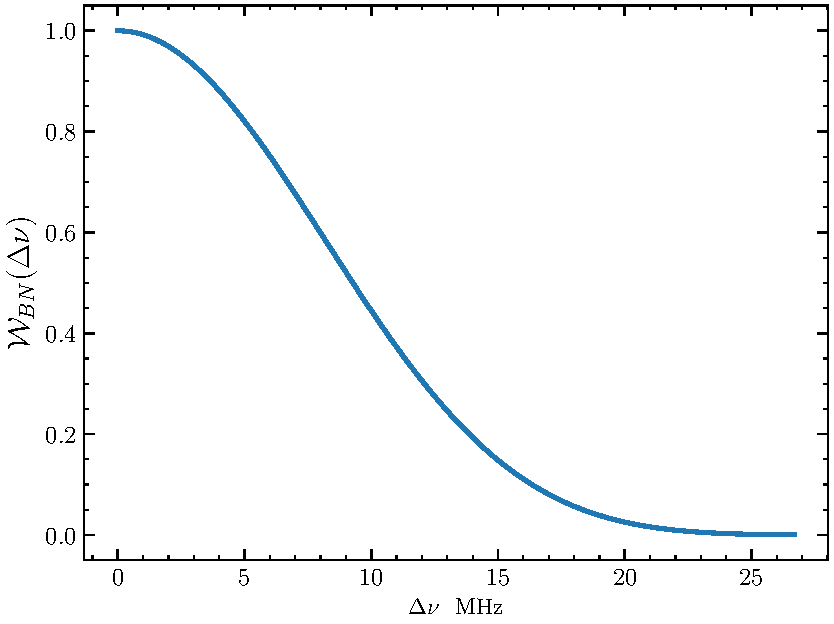
\includegraphics[]{../../../../../Tutorials/others/window.pdf}
\caption{Blackman-Nuttal window function for $N_E=668$ with $\Delta\nu_c = 0.04\,\text{\rm MHz}$.}
\end{figure}

\noindent\rule{\linewidth}{0.4pt}

\newpage

\end{fulllineitems}

\index{func\_pk() (in module psestimation)@\spxentry{func\_pk()}\spxextra{in module psestimation}}

\begin{fulllineitems}
\phantomsection\label{\detokenize{psestimation:psestimation.func_pk}}
\pysigstartsignatures
\pysiglinewithargsret{\sphinxcode{\sphinxupquote{psestimation.}}\sphinxbfcode{\sphinxupquote{func\_pk}}}{\sphinxparam{\DUrole{n}{cl}}\sphinxparamcomma \sphinxparam{\DUrole{n}{w}}\sphinxparamcomma \sphinxparam{\DUrole{n}{covi}}\sphinxparamcomma \sphinxparam{\DUrole{n}{vfac}}}{}
\pysigstopsignatures
\sphinxAtStartPar
For each annular bin in \sphinxtitleref{uv} plane with effective multipole value \(\ell_a\), we have :
\begin{equation*}
\begin{split}\mathbf{P_a} &= (\mathbb{A}^\dagger\mathbf{N}_a^{-1}\mathbb{A})^{-1} \mathbb{A}^\dagger\mathbf{N}_a^{-1} \times \mathbf{\left[\mathcal{W} C_{\ell_a}\right]}\\
& = \mathbb{M}\times \mathbf{\left[\mathcal{W}_{BN}\,C_{\ell_a}\right]}\end{split}
\end{equation*}
\sphinxAtStartPar
Where \(\mathbb{A}\) matrix is constructed using \sphinxstylestrong{calc\_A} function, \(\mathcal{W}_{BN}\) is the window function. \(\mathbf{P_a}\) is the cylindrical power spectrum value for fixed value of \(k_{\perp a} = \ell_a/r\). In marix notation we can write :
\begin{equation*}
\begin{split}\begin{align*}
\small
\left[
\begin{array}{c}
    P(k_{\perp a},k_{\parallel m = 0 })\\
    P(k_{\perp a},k_{\parallel m = 1 })\\
    \vdots\\
    P(k_{\perp a},k_{\parallel m = N_E-1 })\\
\end{array}\right] =
\begin{bmatrix}
    \mathbb{M}_{00} & \mathbb{M}_{01} & \cdots & \mathbb{M}_{0,N_E-1}\\
    \mathbb{M}_{10} & \mathbb{M}_{11} & \cdots & \mathbb{M}_{1,N_E-1}\\
    \vdots & \vdots & \ddots & \vdots \\
    \mathbb{M}_{N_E-1,0} & \mathbb{M}_{N_E-1,1} & \cdots & \mathbb{M}_{N_E-1,N_E-1}\\
\end{bmatrix} \times
\begin{bmatrix}
    \mathcal{W}_{\rm BN}(\Delta\nu_{n=0}) \times C_{\ell_a}(\Delta\nu_{n=0})\\
    \mathcal{W}_{\rm BN}(\Delta\nu_{n=1}) \times C_{\ell_a}(\Delta\nu_{n=1})\\
    \vdots\\
    \mathcal{W}_{\rm BN}(\Delta\nu_{n=N_E-1}) \times C_{\ell_a}(\Delta\nu_{n=N_E -1})\\
\end{bmatrix}
\end{align*}\end{split}
\end{equation*}\begin{quote}\begin{description}
\sphinxlineitem{Parameters}\begin{itemize}
\item {} 
\sphinxAtStartPar
\sphinxstyleliteralstrong{\sphinxupquote{cl}} (\sphinxstyleliteralemphasis{\sphinxupquote{np.ndarray}}) \textendash{} Multi\sphinxhyphen{}angular power spectrum \(C_{\ell}(\Delta\nu)\) (MAPS) array. Shape \((\dots,len(lval),N\!E)\).

\item {} 
\sphinxAtStartPar
\sphinxstyleliteralstrong{\sphinxupquote{w}} (\sphinxstyleliteralemphasis{\sphinxupquote{np.ndarray}}) \textendash{} The window function normalized to \(\Delta\nu = 0\), which is used to avoid discontinuity at the band edges. Shape \((N\!E,)\).

\item {} 
\sphinxAtStartPar
\sphinxstyleliteralstrong{\sphinxupquote{covi}} (\sphinxstyleliteralemphasis{\sphinxupquote{np.ndarray}}) \textendash{} Inverse of diagonal elements of noise covariance matrix \(\mathbf{N}\) estimated from muliple noise only simulations. Shape \((....,len(lval),N\!E)\).

\item {} 
\sphinxAtStartPar
\sphinxstyleliteralstrong{\sphinxupquote{vfac}} (\sphinxstyleliteralemphasis{\sphinxupquote{int}}\sphinxstyleliteralemphasis{\sphinxupquote{ or }}\sphinxstyleliteralemphasis{\sphinxupquote{float}}) \textendash{} The volume factor \(r^2r'\Delta\nu_c(N\!E-1)\) sitting in the FT of MAPS.

\end{itemize}

\sphinxlineitem{Returns}
\sphinxAtStartPar
\sphinxstylestrong{pk} \textendash{} Cylindrical power spectrum \(P(k_{\perp},k_{\parallel})\) array using MLE (\sphinxstylestrong{maximum likelyhood estimator}). Shape \((....,len(lval),N\!E)\).

\sphinxlineitem{Return type}
\sphinxAtStartPar

\sphinxAtStartPar
np.ndarray
\clearpage

\end{description}\end{quote}
\subsubsection*{Examples}

\begin{sphinxVerbatim}[commandchars=\\\{\}]
\PYG{g+gp}{\PYGZgt{}\PYGZgt{}\PYGZgt{} }\PYG{n}{index} \PYG{o}{=} \PYG{l+m+mi}{7200}
\PYG{g+gp}{\PYGZgt{}\PYGZgt{}\PYGZgt{} }\PYG{n}{cl}   \PYG{o}{=} \PYG{n}{np}\PYG{o}{.}\PYG{n}{load}\PYG{p}{(}\PYG{l+s+sa}{f}\PYG{l+s+s1}{\PYGZsq{}}\PYG{l+s+s1}{/home/cts23ph/git\PYGZus{}package\PYGZus{}myutils/clfuncs/cldnur\PYGZus{}}\PYG{l+s+si}{\PYGZob{}}\PYG{n}{index}\PYG{l+s+si}{\PYGZcb{}}\PYG{l+s+s1}{.npy}\PYG{l+s+s1}{\PYGZsq{}}\PYG{p}{)}\PYG{p}{[}\PYG{o}{.}\PYG{o}{.}\PYG{o}{.}\PYG{p}{,}\PYG{p}{:}\PYG{n}{NE}\PYG{p}{]}
\PYG{g+gp}{\PYGZgt{}\PYGZgt{}\PYGZgt{} }\PYG{n}{cln}  \PYG{o}{=} \PYG{n}{np}\PYG{o}{.}\PYG{n}{load}\PYG{p}{(}\PYG{l+s+sa}{f}\PYG{l+s+s1}{\PYGZsq{}}\PYG{l+s+s1}{/home/cts23ph/git\PYGZus{}package\PYGZus{}myutils/clfuncs/cldnur\PYGZus{}noise\PYGZus{}}\PYG{l+s+si}{\PYGZob{}}\PYG{n}{index}\PYG{l+s+si}{\PYGZcb{}}\PYG{l+s+s1}{.npy}\PYG{l+s+s1}{\PYGZsq{}}\PYG{p}{)}\PYG{p}{[}\PYG{o}{.}\PYG{o}{.}\PYG{o}{.}\PYG{p}{,}\PYG{p}{:}\PYG{n}{NE}\PYG{p}{]}
\PYG{g+gp}{\PYGZgt{}\PYGZgt{}\PYGZgt{} }\PYG{n}{dcln} \PYG{o}{=} \PYG{n}{np}\PYG{o}{.}\PYG{n}{std}\PYG{p}{(}\PYG{n}{cln}\PYG{p}{,} \PYG{n}{axis} \PYG{o}{=} \PYG{l+m+mi}{0}\PYG{p}{)}
\PYG{g+gp}{\PYGZgt{}\PYGZgt{}\PYGZgt{} }\PYG{n}{covi} \PYG{o}{=} \PYG{l+m+mi}{1}\PYG{o}{/}\PYG{n}{dcln}\PYG{o}{*}\PYG{o}{*}\PYG{l+m+mi}{2}
\PYG{g+gp}{\PYGZgt{}\PYGZgt{}\PYGZgt{} }\PYG{c+c1}{\PYGZsh{} window for Fourier transform}
\PYG{g+gp}{\PYGZgt{}\PYGZgt{}\PYGZgt{} }\PYG{n}{w}    \PYG{o}{=} \PYG{n}{pe}\PYG{o}{.}\PYG{n}{window}\PYG{p}{(}\PYG{n}{NE}\PYG{p}{)}
\PYG{g+gp}{\PYGZgt{}\PYGZgt{}\PYGZgt{} }\PYG{c+c1}{\PYGZsh{} MLE cylindrical PS P(kper, kpara)}
\PYG{g+gp}{\PYGZgt{}\PYGZgt{}\PYGZgt{} }\PYG{n}{pk}   \PYG{o}{=} \PYG{n}{pe}\PYG{o}{.}\PYG{n}{func\PYGZus{}pk}\PYG{p}{(}\PYG{n}{cl}\PYG{p}{,} \PYG{n}{w}\PYG{p}{,} \PYG{n}{covi}\PYG{p}{,} \PYG{n}{vfac}\PYG{p}{)}
\PYG{g+gp}{\PYGZgt{}\PYGZgt{}\PYGZgt{} }\PYG{n+nb}{print}\PYG{p}{(}\PYG{l+s+sa}{f}\PYG{l+s+s1}{\PYGZsq{}}\PYG{l+s+si}{\PYGZob{}}\PYG{n}{cl}\PYG{o}{.}\PYG{n}{shape}\PYG{+w}{        }\PYG{l+s+si}{= \PYGZcb{}}\PYG{l+s+se}{\PYGZbs{}}
\PYG{g+gp}{... }\PYG{l+s+s1}{      }\PYG{l+s+se}{\PYGZbs{}n}\PYG{l+s+si}{\PYGZob{}}\PYG{n}{covi}\PYG{o}{.}\PYG{n}{shape}\PYG{+w}{      }\PYG{l+s+si}{= \PYGZcb{}}\PYG{l+s+se}{\PYGZbs{}}
\PYG{g+gp}{... }\PYG{l+s+s1}{      }\PYG{l+s+se}{\PYGZbs{}n}\PYG{l+s+si}{\PYGZob{}}\PYG{n}{w}\PYG{o}{.}\PYG{n}{shape}\PYG{+w}{         }\PYG{l+s+si}{= \PYGZcb{}}\PYG{l+s+se}{\PYGZbs{}}
\PYG{g+gp}{... }\PYG{l+s+s1}{      }\PYG{l+s+se}{\PYGZbs{}n}\PYG{l+s+si}{\PYGZob{}}\PYG{n}{pk}\PYG{o}{.}\PYG{n}{shape}\PYG{+w}{        }\PYG{l+s+si}{= \PYGZcb{}}\PYG{l+s+s1}{\PYGZsq{}}\PYG{p}{)}
\PYG{g+go}{cl.shape        = (20, 668)}
\PYG{g+go}{covi.shape      = (20, 668)}
\PYG{g+go}{w.shape         = (668,)}
\PYG{g+go}{pk.shape        = (20, 668)}
\end{sphinxVerbatim}
\subsubsection*{Notes}

\sphinxAtStartPar
Here we have assumed that the noise covariance matrix \(\mathbf{N}\) is diagonal along frequency separation axis \(\Delta\nu\) and for each annnular bin \(\ell_a\) bin we have :
\begin{equation*}
\begin{split}\left(\mathbf{N_a}\right)_{mn} = \delta_{mn}\, \left[\delta C_{\ell_a}\left(\Delta\nu_n\right)\right]_{\rm noise}^2\end{split}
\end{equation*}
\sphinxAtStartPar
So each element of \sphinxcode{\sphinxupquote{covi}} (the last axis) contains the value \(1/\left[\delta C_{\ell_a}\left(\Delta\nu_n\right)\right]_{\rm noise}^2\).

\sphinxAtStartPar
The explicit form of the marix \(\mathbf{N_a}\) is given as :
\begin{equation*}
\begin{split}\begin{bmatrix}
    \left[\delta C_{\ell_a}\left(\Delta\nu_{n=0}\right)\right]_{\rm noise}^2& 0 & \cdots & 0\\
    0 & \left[\delta C_{\ell_a}\left(\Delta\nu_{n=1}\right)\right]_{\rm noise}^2 & \cdots & 0\\
    \vdots & \vdots & \ddots & \vdots \\
    0 & 0 & \cdots & \left[\delta C_{\ell_a}\left(\Delta\nu_{n=N_E-1}\right)\right]_{\rm noise}^2\\
\end{bmatrix}\end{split}
\end{equation*}
\begin{figure}[H]
\centering
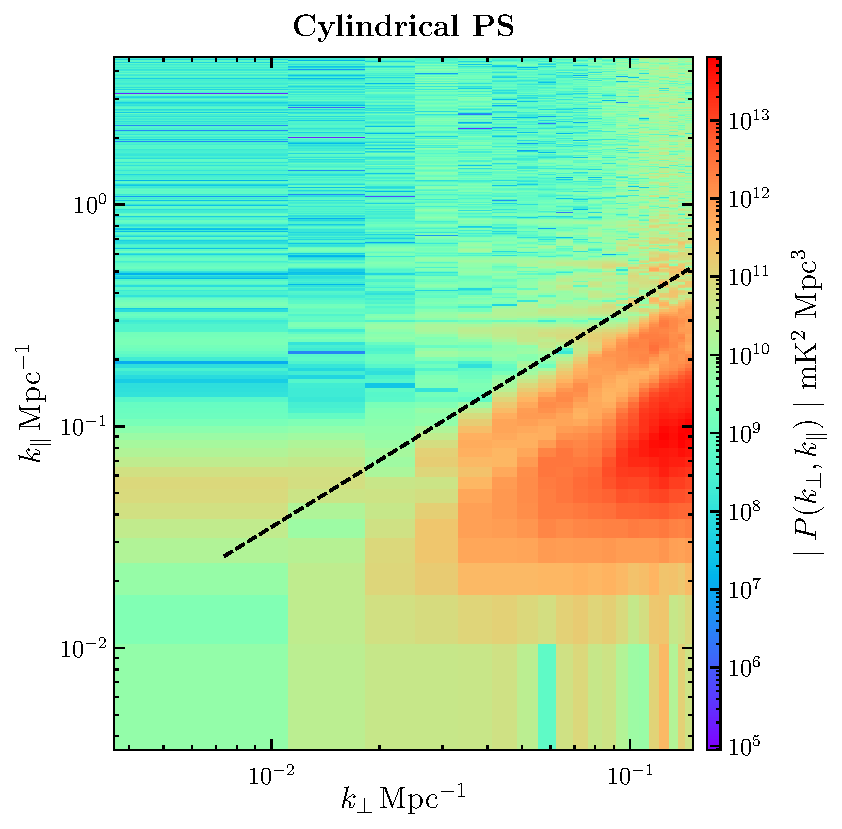
\includegraphics[]{../../../../../Tutorials/others/cyl_ps_7200.pdf}
\caption{Cylindrical Power Spectrum $P(k_\perp,k_\parallel)$.}
\end{figure}

\newpage

\end{fulllineitems}

\index{X() (in module psestimation)@\spxentry{X()}\spxextra{in module psestimation}}

\begin{fulllineitems}
\phantomsection\label{\detokenize{psestimation:psestimation.X}}
\pysigstartsignatures
\pysiglinewithargsret{\sphinxcode{\sphinxupquote{psestimation.}}\sphinxbfcode{\sphinxupquote{X}}}{\sphinxparam{\DUrole{n}{pk}}\sphinxparamcomma \sphinxparam{\DUrole{n}{dpkn}}\sphinxparamcomma \sphinxparam{\DUrole{n}{flag\_mask}}}{}
\pysigstopsignatures\begin{quote}\begin{description}
\sphinxlineitem{Parameters}\begin{itemize}
\item {} 
\sphinxAtStartPar
\sphinxstyleliteralstrong{\sphinxupquote{pk}} (\sphinxstyleliteralemphasis{\sphinxupquote{np.ndarray}}) \textendash{} Cylindrical power spectrum \(P(k_{\perp},k_{\parallel})\) array (\sphinxstylestrong{2D or higher dimensional array}), Must be of shape \([\dots,len(kper),len(kpara)]\).

\item {} 
\sphinxAtStartPar
\sphinxstyleliteralstrong{\sphinxupquote{dpkn}} (\sphinxstyleliteralemphasis{\sphinxupquote{np.ndarray}}) \textendash{} Standard deviation of cylindrical power spectrum \(\delta P_N(k_{\perp},k_{\parallel}) = \sqrt{\langle\left[ P_N(k)\right]^2\rangle - \left\langle P_N(k) \right\rangle^2}\), estimated from noise only simulations. Where \(\langle\cdots\rangle\) denotes average over realizations and \(P_N(k_{\perp},k_{\parallel})\) is the cylindrical power spectrum obtained using noise only simulations. \sphinxstylestrong{Must have same shape as} \sphinxcode{\sphinxupquote{pk}}.

\item {} 
\sphinxAtStartPar
\sphinxstyleliteralstrong{\sphinxupquote{flag\_mask}} (\sphinxstyleliteralemphasis{\sphinxupquote{np.ndarray}}) \textendash{} A \sphinxstylestrong{2D} boolean mask of shape \([len(kper),len(kpara)]\). If the element value is \sphinxstylestrong{1} then that \((k_{\perp},k_{\parallel})\) \sphinxstylestrong{mode is used}, if \sphinxstylestrong{0} then \sphinxstylestrong{rejected}. Should contain values \sphinxstylestrong{0 and 1 only}.

\end{itemize}

\sphinxlineitem{Returns}
\sphinxAtStartPar
\begin{itemize}
\item {} 
\sphinxAtStartPar
\sphinxstylestrong{X} (\sphinxstyleemphasis{np.ndarray}) \textendash{} The values of variable \(X = \dfrac{P(k_{\perp},k_{\parallel})}{\delta P_N(k_{\perp},k_{\parallel})}\) (\sphinxstylestrong{flattened array along last two dimensons}) corresponding to those \((k_{\perp},k_{\parallel})\) modes defined via \sphinxstylestrong{flag\_mask} boolean array. Shape \([\dots,modes]\). Where \sphinxtitleref{modes} is the number of elements containing \sphinxstylestrong{1} in \sphinxstylestrong{flag\_mask} array.

\item {} 
\sphinxAtStartPar
\sphinxstylestrong{mu\_est} (\sphinxstyleemphasis{float  or np.ndarray}) \textendash{} Mean value of \(X\) (\(\mu_{\rm Est}\)) , estimated using \((k_{\perp},k_{\parallel})\) modes defined in \sphinxstylestrong{flag\_mask} boolean array. Shape \(pk.shape[:-2]\). \sphinxstylestrong{last two axes are removed}.

\item {} 
\sphinxAtStartPar
\sphinxstylestrong{sigma\_est} (\sphinxstyleemphasis{float  or np.ndarray}) \textendash{} Standard deviation of \(X\) (\(\sigma_{\rm Est}\)) , estimated using \((k_{\perp},k_{\parallel})\) modes defined in \sphinxstylestrong{flag\_mask} boolean array. Same shape as \sphinxcode{\sphinxupquote{mu\_est}}.

\end{itemize}


\end{description}\end{quote}
\subsubsection*{Examples}

\begin{sphinxVerbatim}[commandchars=\\\{\}]
\PYG{g+gp}{\PYGZgt{}\PYGZgt{}\PYGZgt{} }\PYG{c+c1}{\PYGZsh{} Noise Power Spectrum}
\PYG{g+gp}{\PYGZgt{}\PYGZgt{}\PYGZgt{} }\PYG{c+c1}{\PYGZsh{} MLE cylindrical PS P(kper, kpara)       \PYGZsh{} noise}
\PYG{g+gp}{\PYGZgt{}\PYGZgt{}\PYGZgt{} }\PYG{n}{pkn}   \PYG{o}{=} \PYG{n}{pe}\PYG{o}{.}\PYG{n}{func\PYGZus{}pk}\PYG{p}{(}\PYG{n}{cln}\PYG{p}{,} \PYG{n}{w}\PYG{p}{,} \PYG{n}{covi}\PYG{p}{,} \PYG{n}{vfac}\PYG{p}{)}    \PYG{c+c1}{\PYGZsh{} noise ps}
\PYG{g+gp}{\PYGZgt{}\PYGZgt{}\PYGZgt{} }\PYG{n}{dpkn}  \PYG{o}{=} \PYG{n}{np}\PYG{o}{.}\PYG{n}{std}\PYG{p}{(}\PYG{n}{pkn}\PYG{p}{,} \PYG{n}{axis} \PYG{o}{=} \PYG{l+m+mi}{0}\PYG{p}{)}             \PYG{c+c1}{\PYGZsh{} std noise of ps}
\PYG{g+gp}{\PYGZgt{}\PYGZgt{}\PYGZgt{} }\PYG{n}{dpkn} \PYG{o}{*}\PYG{o}{=} \PYG{p}{(}\PYG{l+m+mi}{20}\PYG{p}{)}\PYG{o}{*}\PYG{o}{*}\PYG{l+m+mi}{2}                           \PYG{c+c1}{\PYGZsh{} scale the noise accordingly}
\PYG{g+gp}{\PYGZgt{}\PYGZgt{}\PYGZgt{} }\PYG{c+c1}{\PYGZsh{} flag mask array}
\PYG{g+gp}{\PYGZgt{}\PYGZgt{}\PYGZgt{} }\PYG{n}{fm} \PYG{o}{=} \PYG{n}{np}\PYG{o}{.}\PYG{n}{load}\PYG{p}{(}\PYG{l+s+s1}{\PYGZsq{}}\PYG{l+s+s1}{/home/cts23ph/git\PYGZus{}package\PYGZus{}myutils/psfuncs/flag\PYGZus{}mask.npy}\PYG{l+s+s1}{\PYGZsq{}}\PYG{p}{)}
\PYG{g+gp}{\PYGZgt{}\PYGZgt{}\PYGZgt{} }\PYG{n+nb}{print}\PYG{p}{(}\PYG{l+s+sa}{f}\PYG{l+s+s1}{\PYGZsq{}}\PYG{l+s+si}{\PYGZob{}}\PYG{n}{pkn}\PYG{o}{.}\PYG{n}{shape}\PYG{+w}{       }\PYG{l+s+si}{= \PYGZcb{}}\PYG{l+s+se}{\PYGZbs{}}
\PYG{g+gp}{... }\PYG{l+s+s1}{      }\PYG{l+s+se}{\PYGZbs{}n}\PYG{l+s+si}{\PYGZob{}}\PYG{n}{dpkn}\PYG{o}{.}\PYG{n}{shape}\PYG{+w}{      }\PYG{l+s+si}{= \PYGZcb{}}\PYG{l+s+se}{\PYGZbs{}}
\PYG{g+gp}{... }\PYG{l+s+s1}{      }\PYG{l+s+se}{\PYGZbs{}n}\PYG{l+s+si}{\PYGZob{}}\PYG{n}{fm}\PYG{o}{.}\PYG{n}{shape}\PYG{+w}{        }\PYG{l+s+si}{= \PYGZcb{}}\PYG{l+s+s1}{\PYGZsq{}}\PYG{p}{)}
\PYG{g+go}{pkn.shape       = (50, 20, 668)}
\PYG{g+go}{dpkn.shape      = (20, 668)}
\PYG{g+go}{fm.shape        = (20, 668)}
\PYG{g+gp}{\PYGZgt{}\PYGZgt{}\PYGZgt{} }\PYG{n}{X}\PYG{p}{,} \PYG{n}{mu}\PYG{p}{,} \PYG{n}{sigma} \PYG{o}{=} \PYG{n}{pe}\PYG{o}{.}\PYG{n}{X}\PYG{p}{(}\PYG{n}{pk}\PYG{p}{,} \PYG{n}{dpkn}\PYG{p}{,} \PYG{n}{fm}\PYG{p}{)} \PYG{c+c1}{\PYGZsh{} X statistics}
\PYG{g+gp}{\PYGZgt{}\PYGZgt{}\PYGZgt{} }\PYG{n}{np}\PYG{o}{.}\PYG{n}{set\PYGZus{}printoptions}\PYG{p}{(}\PYG{n}{precision} \PYG{o}{=} \PYG{l+m+mi}{3}\PYG{p}{,} \PYG{n}{suppress} \PYG{o}{=} \PYG{k+kc}{True}\PYG{p}{)}
\PYG{g+gp}{\PYGZgt{}\PYGZgt{}\PYGZgt{} }\PYG{n+nb}{print}\PYG{p}{(}\PYG{l+s+sa}{f}\PYG{l+s+s1}{\PYGZsq{}}\PYG{l+s+si}{\PYGZob{}}\PYG{n}{X}\PYG{o}{.}\PYG{n}{shape}\PYG{+w}{ }\PYG{l+s+si}{= \PYGZcb{}}\PYG{l+s+se}{\PYGZbs{}}
\PYG{g+gp}{... }\PYG{l+s+s1}{       }\PYG{l+s+se}{\PYGZbs{}n}\PYG{l+s+s1}{mu      = }\PYG{l+s+si}{\PYGZob{}}\PYG{n}{mu}\PYG{l+s+si}{\PYGZcb{}}\PYG{l+s+se}{\PYGZbs{}}
\PYG{g+gp}{... }\PYG{l+s+s1}{       }\PYG{l+s+se}{\PYGZbs{}n}\PYG{l+s+s1}{sigma   = }\PYG{l+s+si}{\PYGZob{}}\PYG{n}{sigma}\PYG{l+s+si}{\PYGZcb{}}\PYG{l+s+s1}{\PYGZsq{}}\PYG{p}{)}
\PYG{g+go}{X.shape = (503,)}
\PYG{g+go}{mu      = 0.2797964155866535}
\PYG{g+go}{sigma   = 1.2258385055783663}
\end{sphinxVerbatim}

\begin{figure}[H]
\centering
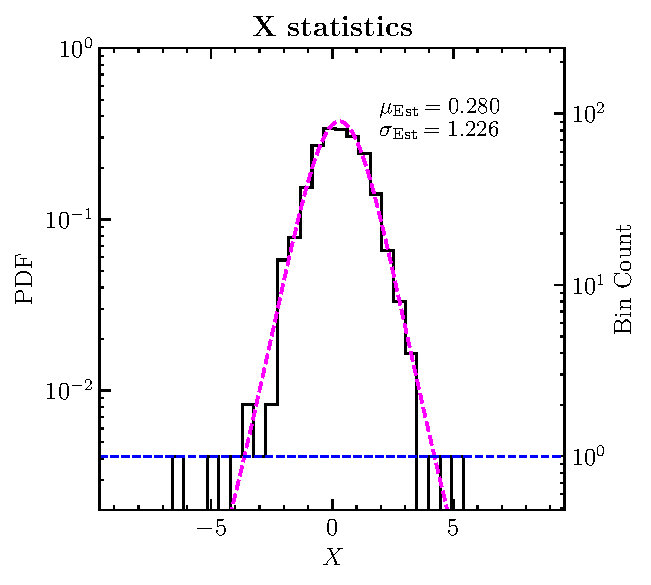
\includegraphics[]{../../../../../Tutorials/others/X_7200.pdf}
\caption{X statistics. The magenta colored line shows student t fit.}
\end{figure}
\subsubsection*{Notes}

\sphinxAtStartPar
Here is how you can make flag mask array.

\begin{sphinxVerbatim}[commandchars=\\\{\}]
\PYG{o}{\PYGZgt{}\PYGZgt{}} \PYG{n}{flag\PYGZus{}mask} \PYG{o}{=} \PYG{n}{np}\PYG{o}{.}\PYG{n}{zeros}\PYG{p}{(}\PYG{p}{(}\PYG{n}{kper}\PYG{o}{.}\PYG{n}{size}\PYG{p}{,}\PYG{n}{kpara}\PYG{o}{.}\PYG{n}{size}\PYG{p}{)}\PYG{p}{,} \PYG{n}{dtype} \PYG{o}{=} \PYG{l+s+s1}{\PYGZsq{}}\PYG{l+s+s1}{int}\PYG{l+s+s1}{\PYGZsq{}}\PYG{p}{)}
\PYG{o}{\PYGZgt{}\PYGZgt{}} \PYG{n+nb}{print}\PYG{p}{(}\PYG{n}{flag\PYGZus{}mask}\PYG{o}{.}\PYG{n}{shape}\PYG{p}{)}
\PYG{o}{\PYGZgt{}\PYGZgt{}} \PYG{n}{ks}  \PYG{o}{=} \PYG{n}{np}\PYG{o}{.}\PYG{n}{array}\PYG{p}{(}\PYG{p}{[}\PYG{l+m+mf}{0.135}\PYG{p}{,} \PYG{l+m+mf}{0.228}\PYG{p}{,} \PYG{l+m+mf}{0.36}\PYG{p}{,} \PYG{l+m+mf}{0.5}\PYG{p}{,} \PYG{l+m+mf}{0.72}\PYG{p}{,} \PYG{l+m+mf}{0.8}\PYG{p}{,} \PYG{l+m+mf}{0.92}\PYG{p}{,} \PYG{l+m+mf}{1.09}\PYG{p}{,} \PYG{l+m+mf}{1.17}\PYG{p}{,} \PYG{l+m+mf}{1.39}\PYG{p}{]}\PYG{p}{)}
\PYG{o}{\PYGZgt{}\PYGZgt{}} \PYG{n}{ksv} \PYG{o}{=} \PYG{n}{np}\PYG{o}{.}\PYG{n}{array}\PYG{p}{(}\PYG{p}{[}\PYG{l+m+mi}{0}\PYG{p}{,}\PYG{l+m+mi}{0}\PYG{p}{,}\PYG{l+m+mi}{1}\PYG{p}{,}\PYG{l+m+mi}{2}\PYG{p}{,}\PYG{l+m+mi}{2}\PYG{p}{,}\PYG{l+m+mi}{2}\PYG{p}{]}\PYG{p}{)}
\PYG{o}{\PYGZgt{}\PYGZgt{}} \PYG{k}{for} \PYG{n}{ii} \PYG{o+ow}{in} \PYG{n+nb}{range}\PYG{p}{(}\PYG{n+nb}{len}\PYG{p}{(}\PYG{n}{ksv}\PYG{p}{)}\PYG{p}{)}\PYG{p}{:}
\PYG{o}{\PYGZgt{}\PYGZgt{}}     \PYG{k}{for} \PYG{n}{jj} \PYG{o+ow}{in} \PYG{n+nb}{range}\PYG{p}{(}\PYG{n}{ksv}\PYG{p}{[}\PYG{n}{ii}\PYG{p}{]}\PYG{p}{,}\PYG{n+nb}{len}\PYG{p}{(}\PYG{n}{ksv}\PYG{p}{)}\PYG{o}{\PYGZhy{}}\PYG{l+m+mi}{1}\PYG{p}{)}\PYG{p}{:}
\PYG{o}{\PYGZgt{}\PYGZgt{}}         \PYG{n}{mask} \PYG{o}{=} \PYG{p}{(}\PYG{n}{kpara}\PYG{o}{\PYGZgt{}}\PYG{o}{=}\PYG{n}{ks}\PYG{p}{[}\PYG{l+m+mi}{2}\PYG{o}{*}\PYG{n}{jj}\PYG{p}{]}\PYG{p}{)}\PYG{o}{*}\PYG{p}{(}\PYG{n}{kpara}\PYG{o}{\PYGZlt{}}\PYG{o}{=}\PYG{n}{ks}\PYG{p}{[}\PYG{l+m+mi}{2}\PYG{o}{*}\PYG{n}{jj}\PYG{o}{+}\PYG{l+m+mi}{1}\PYG{p}{]}\PYG{p}{)}
\PYG{o}{\PYGZgt{}\PYGZgt{}}         \PYG{n}{flag\PYGZus{}mask}\PYG{p}{[}\PYG{n}{ii}\PYG{p}{,}\PYG{n}{mask}\PYG{p}{]} \PYG{o}{=} \PYG{l+m+mi}{1}
\PYG{o}{\PYGZgt{}\PYGZgt{}} \PYG{n}{np}\PYG{o}{.}\PYG{n}{save}\PYG{p}{(}\PYG{l+s+s1}{\PYGZsq{}}\PYG{l+s+s1}{flag\PYGZus{}mask.npy}\PYG{l+s+s1}{\PYGZsq{}}\PYG{p}{,}\PYG{n}{flag\PYGZus{}mask}\PYG{p}{)}   \PYG{c+c1}{\PYGZsh{} save the array}
\end{sphinxVerbatim}

\sphinxAtStartPar
Where the modes used is tabulated below :

\begin{table}
\centering
\setlength{\tabcolsep}{10pt}
\setlength{\arrayrulewidth}{0.5pt}
\renewcommand{\arraystretch}{1.4}
\setlength{\doublerulesep}{1.5pt}  % <-- reduce space between double lines
\resizebox{0.8\textwidth}{!}{
\begin{tabular}{|c|c|c|c|c|c|}
\hline
$k_{\perp}\,\rm Mpc^{-1}$ & \multicolumn{5}{c|}{$k_{\parallel} \,\rm Mpc^{-1}$} \\
\hline
$0.007$ & $0.135-0.228$ & $0.360-0.499$ & $0.720-0.797$ & $0.921-1.095$ & $1.171-1.399$ \\\hline
$0.015$ & $0.135-0.228$ & $0.360-0.499$ & $0.720-0.797$ & $0.921-1.095$ & $1.171-1.399$ \\\hline
$0.022$ & $-$           & $0.360-0.499$ & $0.720-0.797$ & $0.921-1.095$ & $1.171-1.399$ \\\hline
$0.029$ & $-$           & $-$           & $0.720-0.797$ & $0.921-1.095$ & $1.171-1.399$ \\\hline
$0.038$ & $-$           & $-$           & $0.720-0.797$ & $0.921-1.095$ & $1.171-1.399$ \\\hline
$0.045$ & $-$           & $-$           & $0.720-0.797$ & $0.921-1.095$ & $1.171-1.399$ \\\hline
\end{tabular}}
\caption{$k_{\parallel}$ ranges corresponding to different $k_{\perp}$ values that have been used to estimate binned PS and X statistics.}
\label{table:mask}
\end{table}

\end{fulllineitems}

\index{binned\_pk() (in module psestimation)@\spxentry{binned\_pk()}\spxextra{in module psestimation}}

\begin{fulllineitems}
\phantomsection\label{\detokenize{psestimation:psestimation.binned_pk}}
\pysigstartsignatures
\pysiglinewithargsret{\sphinxcode{\sphinxupquote{psestimation.}}\sphinxbfcode{\sphinxupquote{binned\_pk}}}{\sphinxparam{\DUrole{n}{kper}}\sphinxparamcomma \sphinxparam{\DUrole{n}{kpara}}\sphinxparamcomma \sphinxparam{\DUrole{n}{pk}}\sphinxparamcomma \sphinxparam{\DUrole{n}{dpk}}\sphinxparamcomma \sphinxparam{\DUrole{n}{NBin}}\sphinxparamcomma \sphinxparam{\DUrole{n}{flag\_mask}}}{}
\pysigstopsignatures
\sphinxAtStartPar
Using the mode information contained in \sphinxstylestrong{flag\_mask}, first it computes all the \(k\,(={ \sqrt{k_{\perp}^2+k_{\parallel}^2}})\) values available and bins the \((k_{\perp},k_{\parallel})\) space into \(N\!Bin\) no of \sphinxstylestrong{logarithmic bins}. And for each bin \(k_i\), it computes binned power spectrum values \(P(k_i)\) and the corresponding error \(\delta P(k_i)\) using \sphinxstylestrong{the minimum variance estimator}. See notes for more details.
\begin{equation*}
\begin{split}P(k_i) &= \frac{\sum_{(k_\perp,k_\parallel)\in\, i}\,\mathbf{w}(k_{\perp},k_{\parallel})\,P(k_{\perp},k_{\parallel})}{\sum_{(k_\perp,k_\parallel)\in\, i}\,\mathbf{w}(k_{\perp},k_{\parallel})}\\[0.5em]
\delta P(k_i) &= \left[{\sum_{(k_\perp,k_\parallel)\in\, i}\,\mathbf{w}(k_{\perp},k_{\parallel})}\right]^{-1/2}\\[0.5em]
k_i &= \mathbf{exp}\left[\frac{\sum_{(k_\perp,k_\parallel)\in\, i}\,\mathbf{{{w}}}(k_{\perp},k_{\parallel})\,ln(k)}{\sum_{(k_\perp,k_\parallel)\in\, i}\,\mathbf{{{w}}}(k_{\perp},k_{\parallel})}\right];\end{split}
\end{equation*}
\sphinxAtStartPar
Where \(\mathbf{w}(k_{\perp},k_{\parallel})\) is the weight assigned to that particular \((k_{\perp},k_{\parallel})\) mode and by  \((\sum_{k_\perp,k_\parallel})\in \, i\), we denote, the sum is being performed using all the \((k_{\perp},k_{\parallel})\) modes which lies in \(i^{\rm th}\) bin.
\begin{quote}\begin{description}
\sphinxlineitem{Parameters}\begin{itemize}
\item {} 
\sphinxAtStartPar
\sphinxstyleliteralstrong{\sphinxupquote{kper}} (\sphinxstyleliteralemphasis{\sphinxupquote{np.ndarray}}) \textendash{} \sphinxstylestrong{1d array} containing the values of wave\sphinxhyphen{}vector \(\vec{\mathbf{k}}\) \sphinxstylestrong{perpendicular} to the line of sight \sphinxstylestrong{(LOS)}. Denoted by sign \(k_{\perp}\).

\item {} 
\sphinxAtStartPar
\sphinxstyleliteralstrong{\sphinxupquote{kpara}} (\sphinxstyleliteralemphasis{\sphinxupquote{np.ndarray}}) \textendash{} \sphinxstylestrong{1d array} containing the values of wave\sphinxhyphen{}vector \(\vec{\mathbf{k}}\) \sphinxstylestrong{along} to the line of sight \sphinxstylestrong{(LOS)}. Denoted by sign \(k_{\parallel}\).

\item {} 
\sphinxAtStartPar
\sphinxstyleliteralstrong{\sphinxupquote{pk}} (\sphinxstyleliteralemphasis{\sphinxupquote{np.ndarray}}) \textendash{} Cylindrical power spectrum \(P(k_{\perp},k_{\parallel})\) array (\sphinxstylestrong{2D or higher dimensional array}), Must be of shape \([\dots,len(kper),len(kpara)]\).

\item {} 
\sphinxAtStartPar
\sphinxstyleliteralstrong{\sphinxupquote{dpk}} (\sphinxstyleliteralemphasis{\sphinxupquote{np.ndarray}}) \textendash{} Standard deviation of cylindrical noised power spectrum (scaled) \(\delta P_N^{True}(k_{\perp},k_{\parallel}) = \sigma_{\rm Est}\,\delta P_N(k_{\perp},k_{\parallel})\) array (\sphinxstylestrong{2D or higher dimensional array}), Must be of shape \([\dots,len(kper),len(kpara)]\), same shape as \sphinxstylestrong{pk}.

\item {} 
\sphinxAtStartPar
\sphinxstyleliteralstrong{\sphinxupquote{NBin}} (\sphinxstyleliteralemphasis{\sphinxupquote{int}}) \textendash{} No of bins the whole \((k_{\perp},k_{\parallel})\) space has been divided into using only the modes defined in \sphinxstylestrong{flag\_mask} mode info.

\item {} 
\sphinxAtStartPar
\sphinxstyleliteralstrong{\sphinxupquote{flag\_mask}} (\sphinxstyleliteralemphasis{\sphinxupquote{np.ndarray}}) \textendash{} A \sphinxstylestrong{2D} boolean mask of shape \([len(kper),len(kpar–a)]\). If the element value is \sphinxstylestrong{1} then that \((k_{\perp},k_{\parallel})\) \sphinxstylestrong{mode is used}, if \sphinxstylestrong{0} then \sphinxstylestrong{rejected}. Should contain values \sphinxstylestrong{0 and 1 only}.

\end{itemize}

\sphinxlineitem{Returns}
\sphinxAtStartPar
\begin{itemize}
\item {} 
\sphinxAtStartPar
\sphinxstylestrong{keff} (\sphinxstyleemphasis{np.ndarray}) \textendash{} The binned \(k\) values (\sphinxstylestrong{1d array}). Shape \(({nzN\!Bin},)\).

\item {} 
\sphinxAtStartPar
\sphinxstylestrong{ppk} (\sphinxstyleemphasis{np.ndarray}) \textendash{} Binned power spectrum \(P(k)\) values (\sphinxstylestrong{Spherical PS}), (\sphinxstylestrong{n\sphinxhyphen{}dimensional array}). Shape :\((\dots,{nzN\!Bin})\).

\item {} 
\sphinxAtStartPar
\sphinxstylestrong{dppk} (\sphinxstyleemphasis{np.ndarray}) \textendash{} \(1\sigma\) error in estimating spherical ps, \(\delta P(k)\) values, (\sphinxstylestrong{n\sphinxhyphen{}dimensional array}). Shape \((\dots,{nzN\!Bin})\).

\end{itemize}


\end{description}\end{quote}
\subsubsection*{Examples}

\begin{sphinxVerbatim}[commandchars=\\\{\}]
\PYG{g+gp}{\PYGZgt{}\PYGZgt{}\PYGZgt{} }\PYG{n}{NBin} \PYG{o}{=} \PYG{l+m+mi}{5}
\PYG{g+gp}{\PYGZgt{}\PYGZgt{}\PYGZgt{} }\PYG{n}{kk}\PYG{p}{,} \PYG{n}{ppk}\PYG{p}{,} \PYG{n}{dppk} \PYG{o}{=} \PYG{n}{pe}\PYG{o}{.}\PYG{n}{binned\PYGZus{}pk}\PYG{p}{(}\PYG{n}{kper}\PYG{p}{,} \PYG{n}{kpara}\PYG{p}{,} \PYG{n}{pk}\PYG{p}{,} \PYG{n}{sigma}\PYG{o}{*}\PYG{n}{dpkn}\PYG{p}{,}
\PYG{g+gp}{... }                             \PYG{n}{NBin}\PYG{p}{,} \PYG{n}{fm}\PYG{p}{)}
\PYG{g+go}{Bin count   : [ 26   3  60  96 318]}
\PYG{g+gp}{\PYGZgt{}\PYGZgt{}\PYGZgt{} }\PYG{c+c1}{\PYGZsh{} kk   = binned k values}
\PYG{g+gp}{\PYGZgt{}\PYGZgt{}\PYGZgt{} }\PYG{c+c1}{\PYGZsh{} ppk  = binned P(k) values}
\PYG{g+gp}{\PYGZgt{}\PYGZgt{}\PYGZgt{} }\PYG{c+c1}{\PYGZsh{} dppk = 1 sigma error in estimating binned P(k) values}
\PYG{g+gp}{\PYGZgt{}\PYGZgt{}\PYGZgt{} }\PYG{n+nb}{print}\PYG{p}{(}\PYG{l+s+sa}{f}\PYG{l+s+s1}{\PYGZsq{}}\PYG{l+s+si}{\PYGZob{}}\PYG{n}{kk}\PYG{o}{.}\PYG{n}{shape}\PYG{+w}{    }\PYG{l+s+si}{= \PYGZcb{}}\PYG{l+s+se}{\PYGZbs{}}
\PYG{g+gp}{... }\PYG{l+s+s1}{      }\PYG{l+s+se}{\PYGZbs{}n}\PYG{l+s+si}{\PYGZob{}}\PYG{n}{ppk}\PYG{o}{.}\PYG{n}{shape}\PYG{+w}{   }\PYG{l+s+si}{= \PYGZcb{}}\PYG{l+s+se}{\PYGZbs{}}
\PYG{g+gp}{... }\PYG{l+s+s1}{      }\PYG{l+s+se}{\PYGZbs{}n}\PYG{l+s+si}{\PYGZob{}}\PYG{n}{dppk}\PYG{o}{.}\PYG{n}{shape}\PYG{+w}{  }\PYG{l+s+si}{= \PYGZcb{}}\PYG{l+s+s1}{\PYGZsq{}}\PYG{p}{)}
\PYG{g+go}{kk.shape    = (5,)}
\PYG{g+go}{ppk.shape   = (5,)}
\PYG{g+go}{dppk.shape  = (5,)}
\PYG{g+gp}{\PYGZgt{}\PYGZgt{}\PYGZgt{} }\PYG{n}{NBin} \PYG{o}{=} \PYG{l+m+mi}{8}
\PYG{g+gp}{\PYGZgt{}\PYGZgt{}\PYGZgt{} }\PYG{n}{kk}\PYG{p}{,} \PYG{n}{ppk}\PYG{p}{,} \PYG{n}{dppk} \PYG{o}{=} \PYG{n}{pe}\PYG{o}{.}\PYG{n}{binned\PYGZus{}pk}\PYG{p}{(}\PYG{n}{kper}\PYG{p}{,} \PYG{n}{kpara}\PYG{p}{,} \PYG{n}{pk}\PYG{p}{,} \PYG{n}{sigma}\PYG{o}{*}\PYG{n}{dpkn}\PYG{p}{,}
\PYG{g+gp}{... }                             \PYG{n}{NBin}\PYG{p}{,} \PYG{n}{fm}\PYG{p}{)}
\PYG{g+go}{Bin count   : [ 15  11   0  45  18  72 150 192]}
\PYG{g+gp}{\PYGZgt{}\PYGZgt{}\PYGZgt{} }\PYG{c+c1}{\PYGZsh{} kk   = binned k values}
\PYG{g+gp}{\PYGZgt{}\PYGZgt{}\PYGZgt{} }\PYG{c+c1}{\PYGZsh{} ppk  = binned P(k) values}
\PYG{g+gp}{\PYGZgt{}\PYGZgt{}\PYGZgt{} }\PYG{c+c1}{\PYGZsh{} dppk = 1 sigma error in estimating binned P(k) values}
\PYG{g+gp}{\PYGZgt{}\PYGZgt{}\PYGZgt{} }\PYG{n+nb}{print}\PYG{p}{(}\PYG{l+s+sa}{f}\PYG{l+s+s1}{\PYGZsq{}}\PYG{l+s+si}{\PYGZob{}}\PYG{n}{kk}\PYG{o}{.}\PYG{n}{shape}\PYG{+w}{    }\PYG{l+s+si}{= \PYGZcb{}}\PYG{l+s+se}{\PYGZbs{}}
\PYG{g+gp}{... }\PYG{l+s+s1}{      }\PYG{l+s+se}{\PYGZbs{}n}\PYG{l+s+si}{\PYGZob{}}\PYG{n}{ppk}\PYG{o}{.}\PYG{n}{shape}\PYG{+w}{   }\PYG{l+s+si}{= \PYGZcb{}}\PYG{l+s+se}{\PYGZbs{}}
\PYG{g+gp}{... }\PYG{l+s+s1}{      }\PYG{l+s+se}{\PYGZbs{}n}\PYG{l+s+si}{\PYGZob{}}\PYG{n}{dppk}\PYG{o}{.}\PYG{n}{shape}\PYG{+w}{  }\PYG{l+s+si}{= \PYGZcb{}}\PYG{l+s+s1}{\PYGZsq{}}\PYG{p}{)}
\PYG{g+go}{kk.shape    = (7,)}
\PYG{g+go}{ppk.shape   = (7,)}
\PYG{g+go}{dppk.shape  = (7,)}
\end{sphinxVerbatim}
\subsubsection*{Notes}
\begin{enumerate}
\sphinxsetlistlabels{\arabic}{enumi}{enumii}{}{.}%
\item {} 
\sphinxAtStartPar
If no \((k_{\perp},k_{\parallel})\) mode contibutes to a bin, then we reject those bins in the end.

\item {} 
\sphinxAtStartPar
\({nzN\!Bin}\) is the altered value of number of bins \(N\!Bin\). This happens as it might happen number of modes contuributes is \sphinxstylestrong{zero}.

\item {} 
\sphinxAtStartPar
The binning is performed via the \sphinxstylestrong{minimum\sphinxhyphen{}variance estimator} where we have chosen the weights as :

\end{enumerate}
\begin{equation*}
\begin{split}\mathbf{w}(k_{\perp},k_{\parallel}) = \frac{1}{\left[\delta P_N^{True}(k_{\perp},k_{\parallel})\right]^2} = \frac{1}{\left[\sigma_{\rm Est}\times\delta P_N(k_{\perp},k_{\parallel})\right]^2}\end{split}
\end{equation*}
\clearpage

\end{fulllineitems}

\index{func\_dT() (in module psestimation)@\spxentry{func\_dT()}\spxextra{in module psestimation}}

\begin{fulllineitems}
\phantomsection\label{\detokenize{psestimation:psestimation.func_dT}}
\pysigstartsignatures
\pysiglinewithargsret{\sphinxcode{\sphinxupquote{psestimation.}}\sphinxbfcode{\sphinxupquote{func\_dT}}}{\sphinxparam{\DUrole{n}{kk}}\sphinxparamcomma \sphinxparam{\DUrole{n}{ppk}}\sphinxparamcomma \sphinxparam{\DUrole{n}{dppk}}}{}
\pysigstopsignatures
\sphinxAtStartPar
Given the binned \(k\) values, binned power spectrum \(P(k)\) and it’s \(1\sigma\) error \(\delta P(k)\), it gives the \sphinxstylestrong{dimensionless power spectrum} \(\Delta^2(k)\) and it’s \(2\sigma\) uncertainty, signal to noise ratio \sphinxstylestrong{SNR} and the corresponding \sphinxstylestrong{upper limit} \(\Delta^2_{\text{UL}}(k)\).
\begin{quote}\begin{description}
\sphinxlineitem{Parameters}\begin{itemize}
\item {} 
\sphinxAtStartPar
\sphinxstyleliteralstrong{\sphinxupquote{kk}} (\sphinxstyleliteralemphasis{\sphinxupquote{np.ndarray}}) \textendash{} The binned \(k\) values (\sphinxstylestrong{1d array}). Shape \((len(kk),)\).

\item {} 
\sphinxAtStartPar
\sphinxstyleliteralstrong{\sphinxupquote{ppk}} (\sphinxstyleliteralemphasis{\sphinxupquote{np.ndarray}}) \textendash{} Binned power spectrum \(P(k)\) values, (\sphinxstylestrong{n\sphinxhyphen{}dimensional array}). Shape  \((\dots,len(kk))\).

\item {} 
\sphinxAtStartPar
\sphinxstyleliteralstrong{\sphinxupquote{dppk}} (\sphinxstyleliteralemphasis{\sphinxupquote{np.ndarray}}) \textendash{} \(1\sigma\) error in estimating spherical ps, \(\delta P(k)\) values, (\sphinxstylestrong{n\sphinxhyphen{}dimensional array}). Same shape as \sphinxstylestrong{ppk}.

\end{itemize}

\sphinxlineitem{Returns}
\sphinxAtStartPar
\begin{itemize}
\item {} 
\sphinxAtStartPar
\sphinxstylestrong{dk2} (\sphinxstyleemphasis{np.ndarray}) \textendash{} Dimensionless power spectrum \(\Delta^2(k)\), (\sphinxstylestrong{n\sphinxhyphen{}dimensional array}). Same shape as \sphinxstylestrong{pkk}.

\item {} 
\sphinxAtStartPar
\sphinxstylestrong{dpk2} (\sphinxstyleemphasis{np.ndarray}) \textendash{} Statistical (\(2\sigma\)) error in estimating dimensionless power spectrum \(\Delta^2(k)\), (\sphinxstylestrong{n\sphinxhyphen{}dimensional array}).Same shape as \sphinxstylestrong{pkk}.

\item {} 
\sphinxAtStartPar
\sphinxstylestrong{snr} (\sphinxstyleemphasis{np.ndarray}) \textendash{} Signal to noise ratio. (\sphinxstylestrong{n\sphinxhyphen{}dimensional array}). Same shape as \sphinxstylestrong{pkk}.

\item {} 
\sphinxAtStartPar
\sphinxstylestrong{ul} (\sphinxstyleemphasis{np.ndarray}) \textendash{} Upper limit of dimensionless power spectrum \(\Delta^2_{\text{UL}}(k)\), (\sphinxstylestrong{n\sphinxhyphen{}dimensional array}). Same shape as \sphinxstylestrong{pkk}.

\sphinxAtStartPar
They are defined as follows :
\begin{equation*}
\begin{split} \setlength{\fboxrule}{0.7pt}
 \setlength{\fboxsep}{12pt}     % EXTRA padding
 \fcolorbox{black!0}{gray!0}{$
 \begin{aligned}
 \Delta^2(k)              & = \frac{k^3P(k)}{2\pi^2}\\[0.5em]
 \sigma(k)                & = \frac{k^3\delta P(k)}{2\pi^2}\\[0.5em]
 \textbf{\textsc{SNR}}    & = \Delta^2(k)/\sigma(k) = P(k)/\delta P(k)\\[0.5em]
 \Delta^2_{\text{UL}}(k)  & =
 \begin{cases}
   \Delta^2(k)+2\sigma(k) & \text{if } \Delta^2(k) > 0 \\
   2\sigma(k)             & \text{otherwise}
\end{cases}
\end{aligned}$}\end{split}
\end{equation*}
\item {} 
\sphinxAtStartPar
\sphinxstyleemphasis{.. raw:: latex} \textendash{} newpage

\end{itemize}


\end{description}\end{quote}
\subsubsection*{Examples}

\begin{sphinxVerbatim}[commandchars=\\\{\}]
\PYG{g+gp}{\PYGZgt{}\PYGZgt{}\PYGZgt{} }\PYG{n}{dk2}\PYG{p}{,} \PYG{n}{dpk2}\PYG{p}{,} \PYG{n}{snr}\PYG{p}{,} \PYG{n}{ul} \PYG{o}{=} \PYG{n}{pe}\PYG{o}{.}\PYG{n}{func\PYGZus{}dT}\PYG{p}{(}\PYG{n}{kk}\PYG{p}{,} \PYG{n}{ppk}\PYG{p}{,} \PYG{n}{dppk}\PYG{p}{)}
\PYG{g+gp}{\PYGZgt{}\PYGZgt{}\PYGZgt{} }\PYG{n+nb}{print}\PYG{p}{(}\PYG{l+s+sa}{f}\PYG{l+s+s1}{\PYGZsq{}}\PYG{l+s+si}{\PYGZob{}}\PYG{n}{dk2}\PYG{o}{.}\PYG{n}{shape}\PYG{+w}{   }\PYG{l+s+si}{= \PYGZcb{}}\PYG{l+s+se}{\PYGZbs{}}
\PYG{g+gp}{... }\PYG{l+s+s1}{      }\PYG{l+s+se}{\PYGZbs{}n}\PYG{l+s+si}{\PYGZob{}}\PYG{n}{dpk2}\PYG{o}{.}\PYG{n}{shape}\PYG{+w}{  }\PYG{l+s+si}{= \PYGZcb{}}\PYG{l+s+se}{\PYGZbs{}}
\PYG{g+gp}{... }\PYG{l+s+s1}{      }\PYG{l+s+se}{\PYGZbs{}n}\PYG{l+s+si}{\PYGZob{}}\PYG{n}{snr}\PYG{o}{.}\PYG{n}{shape}\PYG{+w}{   }\PYG{l+s+si}{= \PYGZcb{}}\PYG{l+s+se}{\PYGZbs{}}
\PYG{g+gp}{... }\PYG{l+s+s1}{      }\PYG{l+s+se}{\PYGZbs{}n}\PYG{l+s+si}{\PYGZob{}}\PYG{n}{ul}\PYG{o}{.}\PYG{n}{shape}\PYG{+w}{    }\PYG{l+s+si}{= \PYGZcb{}}\PYG{l+s+s1}{\PYGZsq{}}\PYG{p}{)}
\PYG{g+go}{dk2.shape   = (7,)}
\PYG{g+go}{dpk2.shape  = (7,)}
\PYG{g+go}{snr.shape   = (7,)}
\PYG{g+go}{ul.shape    = (7,)}
\end{sphinxVerbatim}

\begin{figure}[H]
\centering
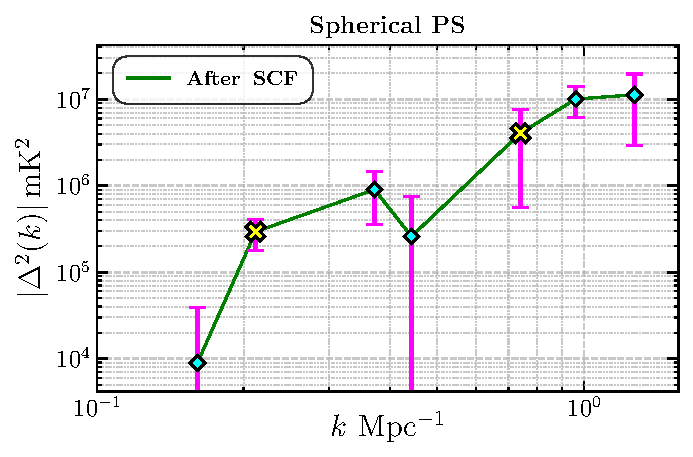
\includegraphics[]{../../../../../Tutorials/others/spheical_ps_7200.pdf}
\caption{Spherical Power Spectrum $P(k)$.}
\end{figure}

\end{fulllineitems}




\renewcommand{\indexname}{Index}
\printindex
\end{document}